\documentclass[a4paper, 12pt]{article}

\usepackage{wrapfig}
\usepackage{graphicx}
\usepackage{mathtext}
\usepackage{amsmath}
\usepackage{siunitx} % Required for alignment
\usepackage{subfigure}
\usepackage{multirow}
\usepackage{rotating}
\usepackage[T1,T2A]{fontenc}
\usepackage[russian]{babel}
\usepackage{caption}

\graphicspath{{pictures/}}


\title{\begin{center}Лабораторная работа №2.2.6\end{center}
Определение энерги активации по температурной зависимости вязкости жидкости}
\author{Гёлецян А.Г.}
\date{\today}

\begin{document}
    \pagenumbering{gobble}
    \maketitle
    \newpage
    \pagenumbering{arabic}


    \textbf{Цель работы:} 1) измерение скорости падения шариков при разной температуре жидкости; 2) вычисление вязксоти жидкости по закону Стокса и расчет энергии активации.

    \textbf{В работе используются:} стеклянный цилиндр с исследуемой жидкостью (глицерин); термостат; секундомер; горизонтальный компаратор; микроскоп; мелкие шарики (диаметром 1-2 мм).

    \section{Теоретическая часть}
    \subsection{Энергия активации}
    Для того чтобы перейти в новое состояние, молекула жидкости должна преодолеть участки с большой потенциальной энергией, превышающей среднюю тепловую энергию молекул. Для этого тепловая энергия молекул должна — вследствие флуктуации — увеличиться на некоторую величину $W$ , называемую энергией активации. Температурная зависимость вязкости жидкости при достаточно грубых предположениях можно опистаь формулой
    \begin{equation} \label{activation_energy:1}
        \eta \sim A e^{W/kT}
    \end{equation}

    Из формулы (\ref{activation_energy:1}) следует, что существует линейня зависимость между величинами $ln\eta$ и $1/T$, и энергию активации можно найти по формуле

    \begin{equation} \label{activation_energy:2}
        W = k \frac{d(ln\eta)}{d(1/T)}
    \end{equation}

    \subsection{Измерение вязкости}
    По формуле Стокса, если шарик радиусом $r$ и со скоростью $v$ движется в среде с вязкостью $\eta$, и при этом не наблюдается турбулентных явлении, тормозящую силу можно найти по формуле (\ref{stokes})

    \begin{equation}\label{stokes}
        F = 6\pi\eta rv
    \end{equation}


    Для измерения вязкости жидкости рассмотрим свободное падение шарика в жидкости. При медленных скоростях на шарик действуют силы Архимеда и Стокса, выражения для которых мы знаем. Отсюда находим выражения для установившейся скорости шарика и вязкости жидкости

        \begin{align}
            v_{уст}&=\frac{2}{9}gr^2\frac{\rho - \rho_ж}{\eta}\label{v_ust}\\
            \eta&=\frac{2}{9}gr^2\frac{\rho - \rho_ж}{v_{уст}}\label{eta}
        \end{align}

    Как видим, измерив установившуюся скорость шарика и параметры системы можно получить вязкость по формуле (\ref{eta}).

    \subsection{Экспериментальная установка}
    Для измерений используется стеклянный цилиндрчиеский сосуд B, наполненный исследуемой жидкостью (глицерин). Диаметр сосуда $\approx 3$ см, длина $\approx 25$ см. На стенках сосуда нанесены две метки на некотором расстоянии друг от друга. Верхняя метка должна располагаться ниже уровня жидкости с таким расчетом, чтобы скорость шарика к моменту прохождения этой метки успевала установиться. Измеряя расстояние между метками, b время падения определяют установившуюся скорость шарика $v_{уст}$. Сам сосуд B помещен в рубашку D, омываемую водой из термостата. При работающем термостате температура воды в рубашке D, а потому и температура жидкости 12 равна температуре воды в термостате.
    Схема прибора (в разрезе) показана на рис.~\ref{ustanovka}.
    \begin{figure}[h]
        \center{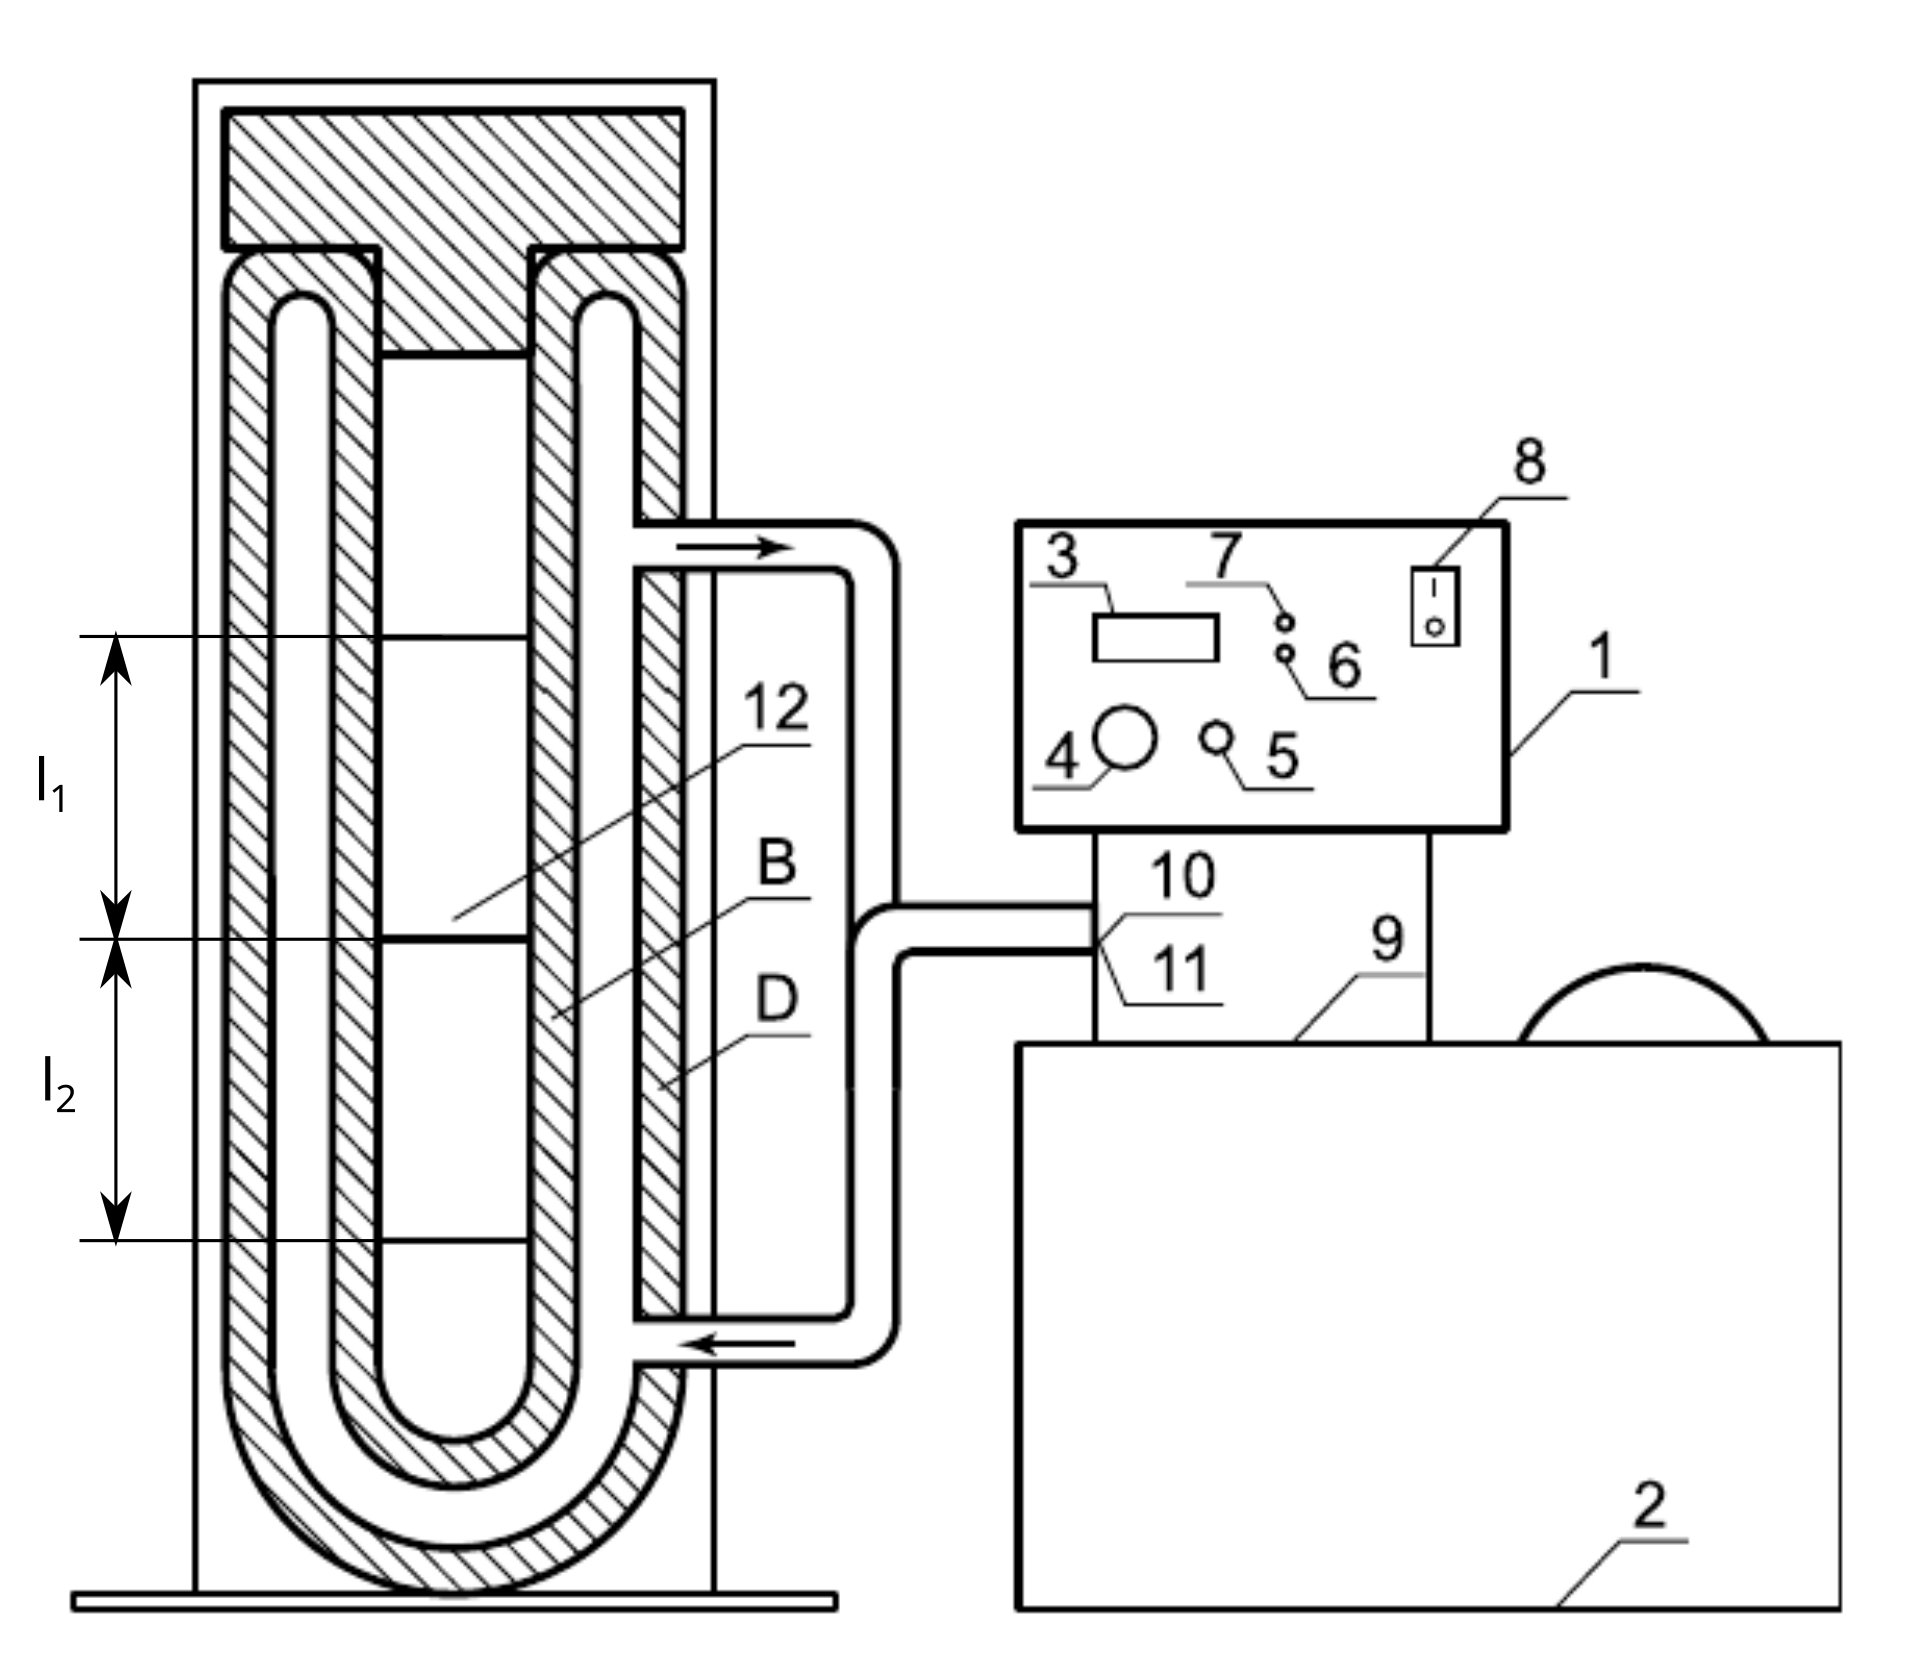
\includegraphics[scale=0.5]{ustanovka}}
        \caption{Установка для определения коэффициента вязкости жидкости.}
        \label{ustanovka}
    \end{figure}


    \section{Ход работы}
    \subsection{Подготовительные работы}
    \begin{figure}[h]
        \center{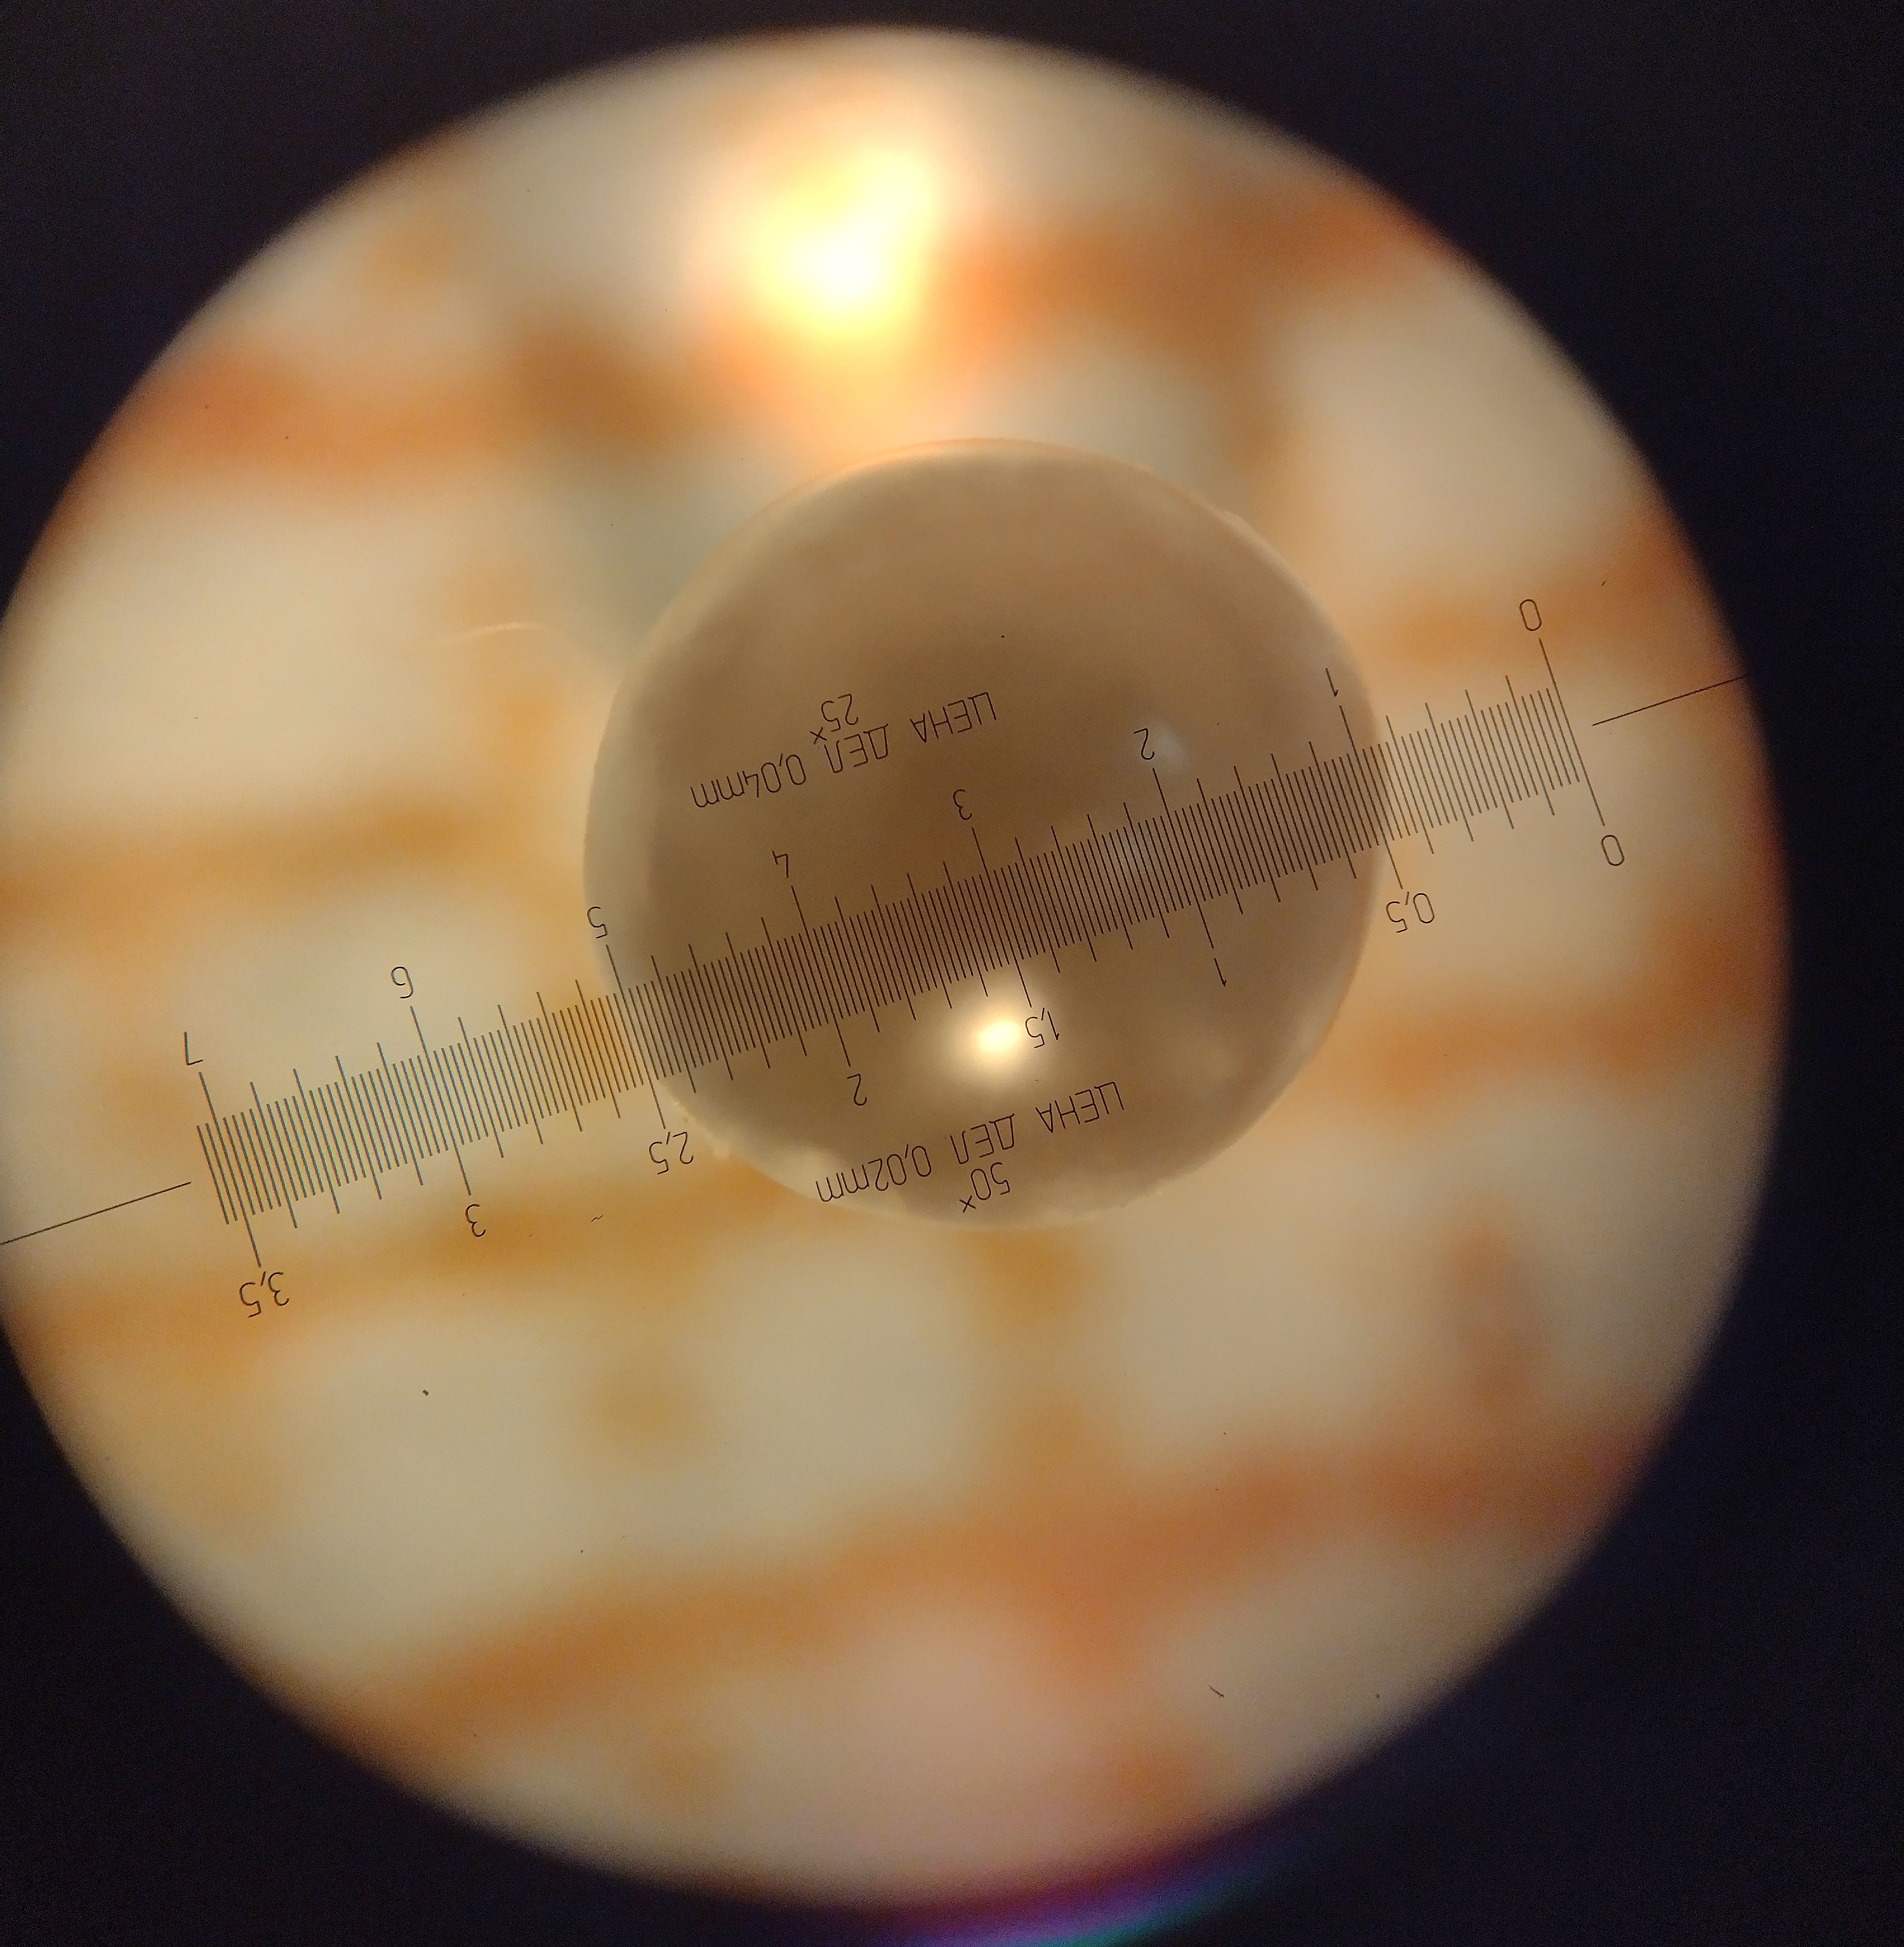
\includegraphics[width=0.7\linewidth]{sharik}}
        \caption{Измерение  диаметра шарика микроскопом.}
        \label{ris:sharik}
    \end{figure}
    Для начала отбираем примерно 25 шариков, и измеряем их диаметры. Диаметры измеряем в трех случайных направлениях и усредняем. Это делается по той причине, что некоторые шарики (в частности металлические) имеют неидеальную геометрию. Данные измерении приведены в таблице \ref{diams}. В таблице шарики с номерами вида $s\#$ стеклянные, а вида $m\#$ металлические. Погрешности измерении диаметров $\sigma_d = 0.02мм$. Плотности шариков в эксперименте

    \begin{align*}
        \rho_{стекло}&=2.5г/см^3\\
        \rho_{металл}&=7.8г/см^3
    \end{align*}

    \newpage

    \begin{table}[h!]
        \vspace{5pt}
        \begin{center}
        \subtable
        {
            \begin{tabular}{|l|rrr|r|}
            \hline
            № &    $d_1$ &    $d_2$ &  $d_3$ & $\langle d \rangle$  \\
              &    мм   &      мм &       мм&         мм\\
            \hline
            s1   &  2.10 &  2.04 &  2.10 &    2.08 \\
            s2   &  2.08 &  2.06 &  2.06 &    2.07 \\
            s3   &  2.10 &  2.10 &  2.10 &    2.10 \\
            s4   &  2.06 &  2.08 &  2.08 &    2.07 \\
            s5   &  2.06 &  2.08 &  2.06 &    2.07 \\
            s6   &  2.08 &  2.08 &  2.08 &    2.08 \\
            s7   &  2.04 &  2.06 &  2.08 &    2.06 \\
            s8   &  2.04 &  2.10 &  2.08 &    2.07 \\
            s9   &  2.10 &  2.08 &  2.06 &    2.08 \\
            s10  &  2.08 &  2.08 &  2.08 &    2.08 \\
            s11  &  2.10 &  2.10 &  2.10 &    2.10 \\
            m1   &  0.66 &  0.70 &  0.70 &    0.69 \\
            m2   &  0.68 &  0.66 &  0.68 &    0.67 \\
            \hline
            \end{tabular}
        }
        \subtable
        {
            \begin{tabular}{|l|rrr|r|}
            \hline
            № &    $d_1$ &    $d_2$ &  $d_3$ & $\langle d \rangle$  \\
              &    мм   &      мм &       мм&         мм\\
            \hline
            m3   &  0.84 &  0.84 &  0.84 &    0.84 \\
            m4   &  0.82 &  0.82 &  0.82 &    0.82 \\
            m5   &  0.76 &  0.76 &  0.76 &    0.76 \\
            m6   &  0.82 &  0.88 &  0.72 &    0.81 \\
            m7   &  0.92 &  0.88 &  0.94 &    0.91 \\
            m8   &  0.88 &  0.92 &  0.88 &    0.89 \\
            m9   &  0.90 &  0.90 &  0.88 &    0.89 \\
            m10  &  0.88 &  0.88 &  0.86 &    0.87 \\
            m11  &  0.96 &  0.92 &  0.92 &    0.93 \\
            m12  &  1.00 &  1.04 &  0.88 &    0.97 \\
            m13  &  0.88 &  0.90 &  0.88 &    0.89 \\
            m14  &  0.94 &  0.98 &  1.00 &    0.97 \\
            m15  &  0.90 &  0.90 &  0.90 &    0.90 \\
                \hline
            \end{tabular}
        }

        \caption{Измеренные диаметры шариков.}
        \label{diams}
        \end{center}
    \end{table}

    Измеряем длины частей цилиндра установки (см. рис. \ref{ustanovka})
    \begin{equation*}
        l_1=l_2=(10.2\pm0.1)см
    \end{equation*}

    \subsection{Измерение установившихся скоростей}
    Мы знаем путь, который проходит шарик от одной отметки цилиндра к другой. Осталось измерить время прохождения между этими отметками для получения скорости. В данной работе время падения определяется изучением видеоматериала, содержащее движение шарика. Для уменьшения ошибки, возникающего вследствие паралакса, камера держится на уровне отметки. Анализировав полученные видеоматериалы получаем следующие данные (см. таблицу \ref{times_in_frames}). Видео снималось с частотой 30 кадров в секунду, следовательно единица времени в таблице $1/30 с$. Как видим $t_1$ и $t_2$ всегда бизки. Отсюда можно предаоложить что на рассматриваемых участках скорость не меняется. В дальнейшем будем считать это предположение правдивым, которое в дальнейшем подтверждается малостью времени и пути релаксации.


    \begin{table}[h!]
        \vspace{5pt}
        \begin{center}
        \subtable
        {
            \begin{tabular}{|l|r|r|r|}
            \hline
            {№} & {$T, ^\circ C$} & {$t_1$} & {$t_2$} \\
            \hline
            s1 & 30.86 & 459 & 452 \\
            s2 & 30.86 & 455 & 453 \\
            s3 & 41.53 & 255 & 252 \\
            s4 & 41.50 & 249 & 250 \\
            s5 & 50.93 & 146 & 150 \\
            s6 & 51.05 & 139 & 146 \\
            s7 & 62.00 & 84 & 88 \\
            s8 & 61.97 & 81 & 87 \\
            s9 & 61.85 & 79 & 81 \\
            s10 & 68.40 & 60 & 61 \\
            s11 & 68.47 & 59 & 61 \\
            \hline
            \end{tabular}
        }
        \subtable
        {
            \begin{tabular}{|l|r|r|r|}
            \hline
            {№} & {$T, ^\circ C$} & {$t_1$} & {$t_2$} \\
            \hline
            m3 & 30.84 & 505 & 507 \\
            m4 & 30.85 & 523 & 523 \\
            m5 & 41.51 & 320 & 313 \\
            m6 & 41.53 & 300 & 302 \\
            m7 & 51.09 & 132 & 135 \\
            m8 & 51.05 & 135 & 143 \\
            m10 & 61.53 & 83 & 81 \\
            m11 & 61.16 & 79 & 78 \\
            m12 & 61.16 & 71 & 71 \\
            m14 & 67.81 & 60 & 59 \\
            m15 & 67.73 & 58 & 60 \\
            \hline
            \end{tabular}
        }

        \caption{Измеренные времена падения шариков в кадрах.}
        \label{times_in_frames}
        \end{center}
    \end{table}
    Для каждого измерения считаем $v$, $\eta$, $Re$, $\tau$, $S$ где $v$ это скорость шарика на участке 1+2, $\tau$ это время релаксации (см. формулу \ref{relaxation_time}), а $S=v\tau$ это путь релаксации.
    \begin{equation}\label{relaxation_time}
        \tau = \frac{2r^2\rho}{9\eta}
    \end{equation}

    Плотность жидкости берем из графика \ref{density}
    \begin{figure}[h]
        \center{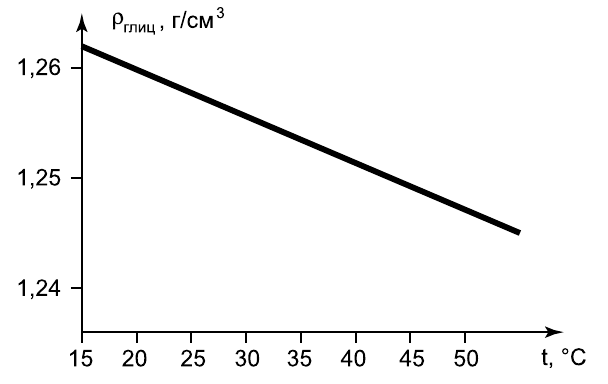
\includegraphics[width=0.7\linewidth]{density}}
        \caption{Плотность глицерина при различных температурах.}
        \label{density}
    \end{figure}
    \paragraph{}
    Данные всех расчетов приведены в таблице \ref{data}

    \newpage

    \begin{table}
    \begin{center}
    \begin{tabular}{|l|l|rr|rr|lll|}
    \hline
    {№} & {$T, ^\circ C$} & {$v, см/с$} & {$\Delta v, см/с$} & {$\eta, мПас$} & {$\Delta\eta, мПас$} & {Re} & {$\tau, мс$} & {$S, \muм$} \\
    \hline
    s1 & 30.86 & 0.67 & 0.007 & 441 & 21 & 0.02 & 0.70 & 0.05 \\
    s2 & 30.86 & 0.67 & 0.007 & 435 & 8 & 0.02 & 0.70 & 0.05 \\
    s3 & 41.53 & 1.20 & 0.012 & 251 & 3 & 0.06 & 1.20 & 0.1 \\
    s4 & 41.50 & 1.21 & 0.013 & 240 & 5 & 0.07 & 1.20 & 0.1 \\
    s5 & 50.93 & 2.05 & 0.023 & 143 & 3 & 0.18 & 2.10 & 0.4 \\
    s6 & 51.05 & 2.13 & 0.024 & 139 & 2 & 0.20 & 2.20 & 0.5 \\
    s7 & 62.00 & 3.52 & 0.045 & 83  & 3 & 0.55 & 3.50 & 1.2 \\
    s8 & 61.97 & 3.61 & 0.047 & 81  & 4 & 0.57 & 3.60 & 1.3 \\
    s9 & 61.85 & 3.79 & 0.05  & 78  & 2 & 0.63 & 3.80 & 1.4 \\
    s10 & 68.40 & 5.01 & 0.077 & 59 & 1 & 1.09 & 5.00 & 2.5 \\
    s11 & 68.47 & 5.05 & 0.078 & 60 & 1 & 1.10 & 5.10 & 2.6 \\\hline
    m3 & 30.84 & 0.60 & 0.006 & 420 & 4 & 0.01 & 0.10 & 0.006 \\
    m4 & 30.85 & 0.58 & 0.006 & 414 & 4 & 0.01 & 0.10 & 0.006 \\
    m5 & 41.51 & 0.96 & 0.01 & 215 & 2 & 0.02 & 0.20 & 0.02 \\
    m6 & 41.53 & 1.01 & 0.01 & 233 & 66 & 0.02 & 0.20 & 0.02 \\
    m7 & 51.09 & 2.27 & 0.025 & 130 & 12 & 0.10 & 0.40 & 0.09 \\
    m8 & 51.05 & 2.18 & 0.024 & 130 & 10 & 0.09 & 0.40 & 0.09 \\
    m10 & 61.53 & 3.70 & 0.049 & 73 & 3 & 0.27 & 0.70 & 0.3 \\
    m11 & 61.16 & 3.86 & 0.052 & 80 & 6 & 0.28 & 0.70 & 0.3 \\
    m12 & 61.16 & 4.27 & 0.06 & 79 & 19 & 0.33 & 0.80 & 0.3 \\
    m14 & 67.81 & 5.09 & 0.079 & 66 & 6 & 0.46 & 1.00 & 0.5 \\
    m15 & 67.73 & 5.14 & 0.08 & 56 & 1 & 0.51 & 1.00 & 0.5 \\
    \hline
    \end{tabular}
    \end{center}

    \caption{Значения вязкостей в экспериментах}
    \label{data}
    \end{table}

    Как видим, времена и пути релаксации очень малые величины, поэтому предположение что установившейся скорость достигается на участках 1 и 2 оправдано. Как видим, числа Рейнольдса в основном меньше 1. Можно предположить что формула Стокса работает, но окончательный вердикт вынесет график зависимости $ln(\eta)(1/T)$. Собственно построим график этой зависимости.

    Построив графики и апроксимировав точки прямой линией методом минимума хи квадрат получаем следующие данные (см. графики в конце)

    \paragraph{}
    Для стеклянных шариков
    \begin{align*}
        W/k &= (5653 \pm 4)К\\
        \bar \chi_{стекло} &= 3.4
    \end{align*}

    Для металлических шариков
    \begin{align*}
        W/k &= (5640 \pm 4)К\\
        \bar \chi_{металл} &= 1.5
    \end{align*}

    Для всех шариков вместе
    \begin{align*}
        W/k &= (5470 \pm 3)К\\
        \bar \chi_{смеш} &= 8.4
    \end{align*}

    Так как у графика со всеми шариками $\bar \chi$ большой, то ее в счет мы не возмьем. Так как у стеклянных шариков ошибки немного занижены ($\bar \chi =3.4$), то учитывая близость значении $W$ для металлических и стеклянных шариков возмьем $W$ как среднее этих двух. Получаем ответ
    \begin{equation}
        W/k = (5647 \pm 4)К
    \end{equation}

    \section{Обсуждение результатов}

    \paragraph{}
    Сравним наши результаты с более точными результатами$^{[1]}$. На графике (4) видно, что значение вязкостей заметно отличаютя при низких температурах, при которых наш метод работает лучше всего. Различие можно обьяснить различием состава глицерина и, возможно, неравномерностью нагрева в нашей установке, т.к. при низких температурах вязкость меняется резче, и неравномерная температура может срьезно повлиять на среднюю вязкость.
    \paragraph{}
    На графике (5), что связь между $ln(\eta)$ и $1/T$ лениейная лишь в некотором приближении. Если попытаться аппроксимировать точки линией методом хи квадрат, то для энергии активации получаем $W/k=(6517\pm2)К$, $\bar \chi = 59.0$. Наша энергия активации отличается от последней на $\varepsilon = 13\%$, что так же можно обьяснить предыдущими аргументами. Значение $\bar\chi$ намекет что линейная модель не описывает данную зависимость.

    \begin{sidewaysfigure}
        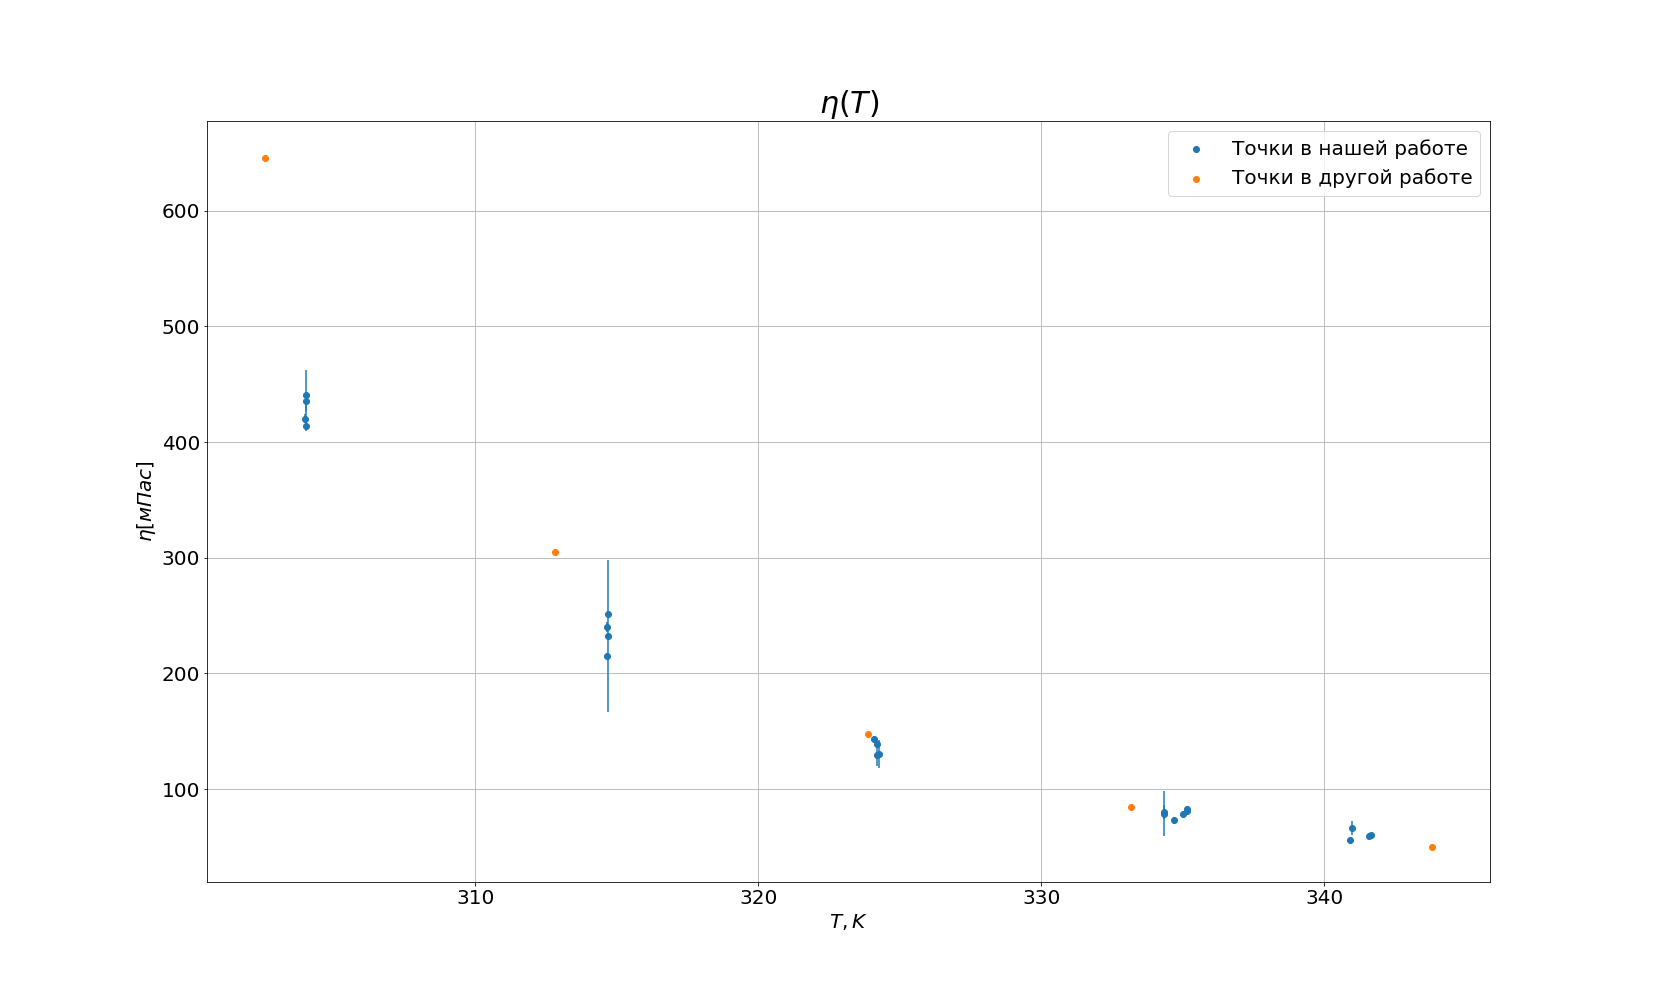
\includegraphics[width=1.2\textwidth]{eta}
        \label{eta_real1}
        \caption{Сравнение вязкостей в разных работах}
    \end{sidewaysfigure}

    \begin{sidewaysfigure}
        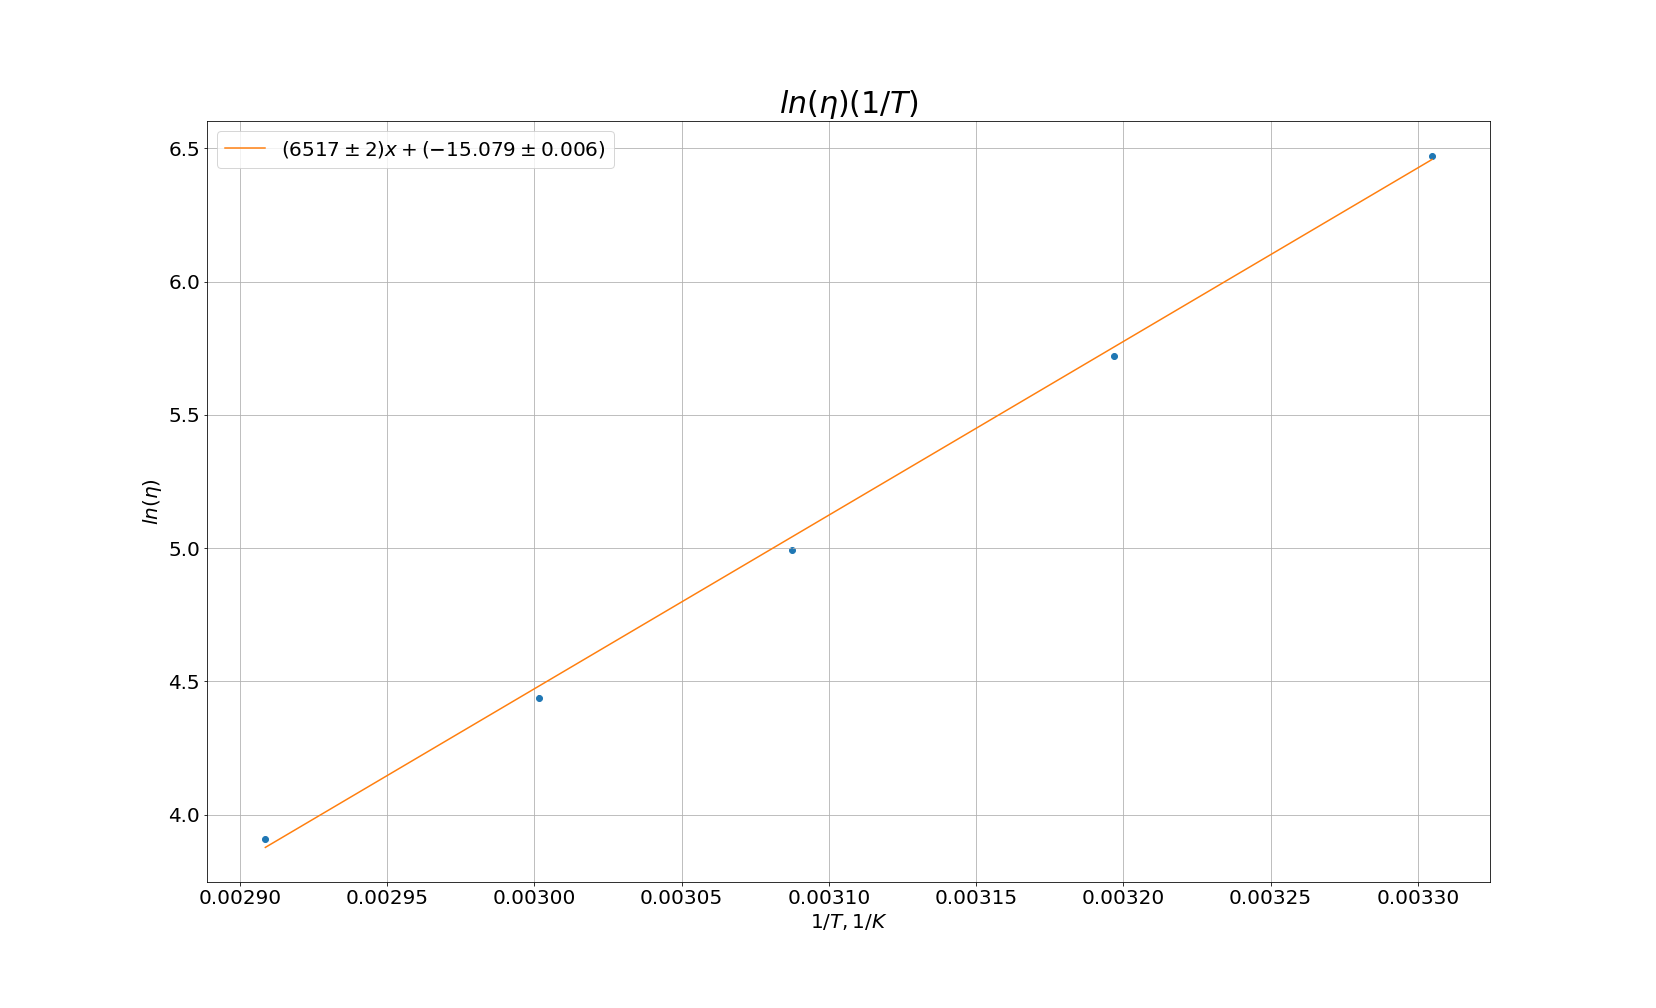
\includegraphics[width=1.2\textwidth]{real}
        \label{eta_real2}
        \caption{Линеаризованный график для данных из работы $[1]$}
    \end{sidewaysfigure}

    \begin{sidewaysfigure}
        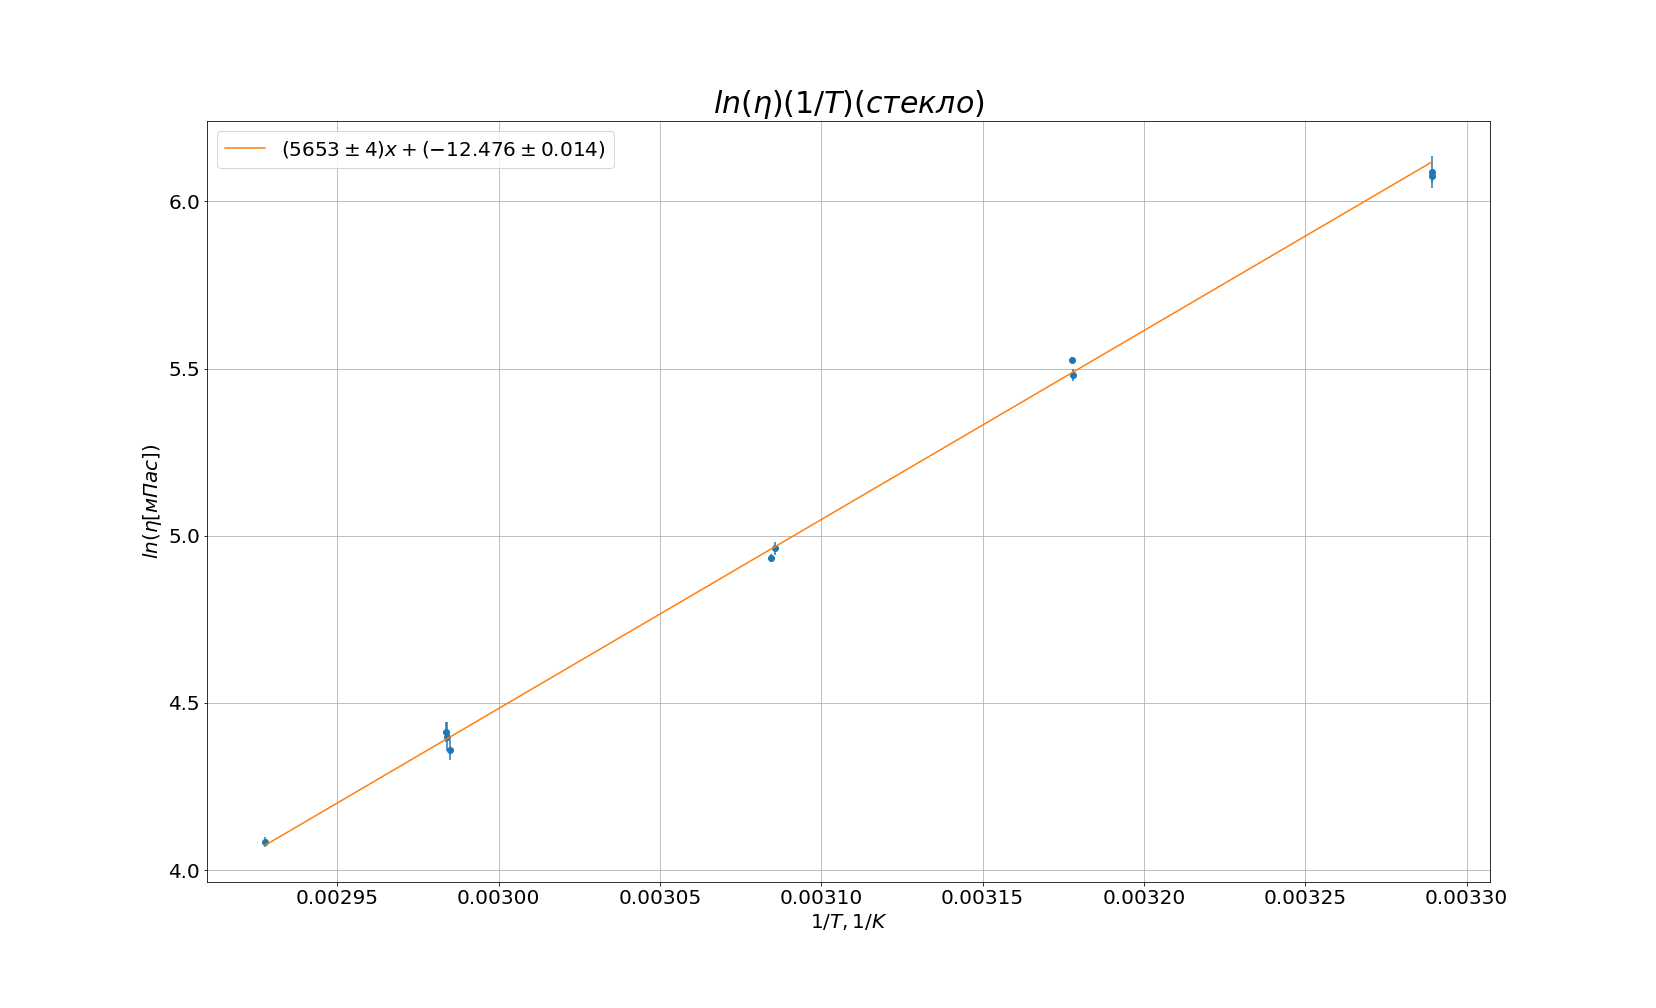
\includegraphics[width=1.2\textwidth]{steklo}
        \label{plot_steklo}
        \caption{График со стеклянными шариками}
    \end{sidewaysfigure}


    \begin{sidewaysfigure}
        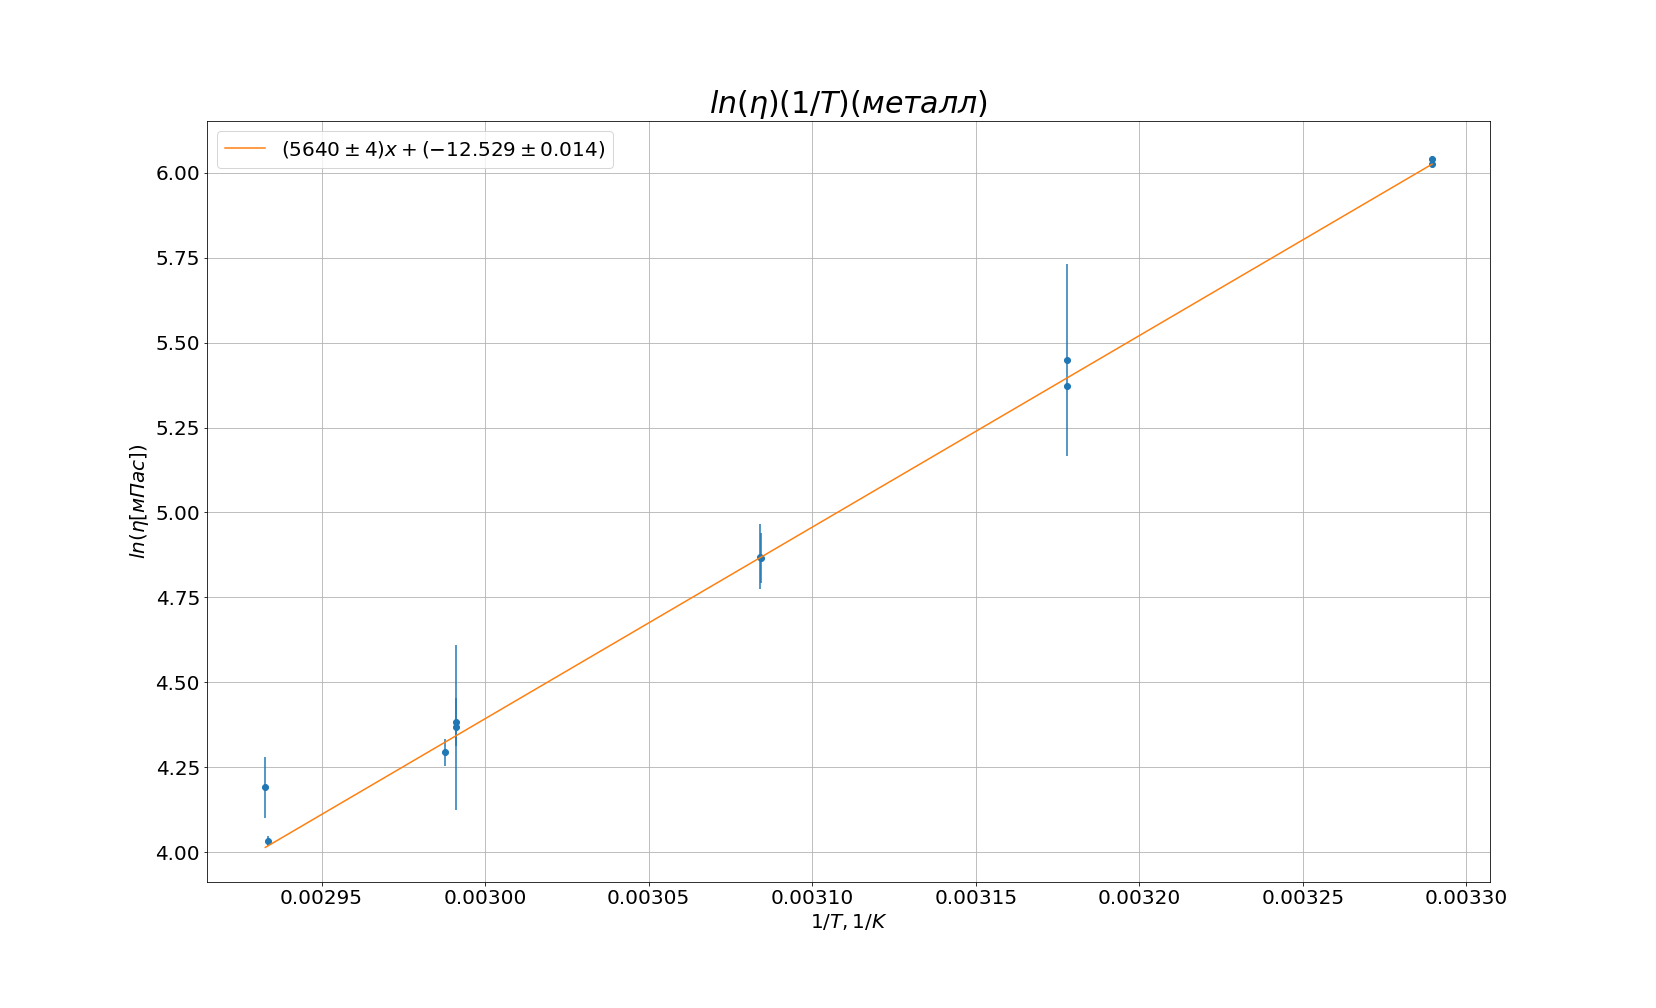
\includegraphics[width=1.2\textwidth]{metal}
        \label{plot_metal}
        \caption{График с металлическими шариками}
    \end{sidewaysfigure}


    \begin{sidewaysfigure}
        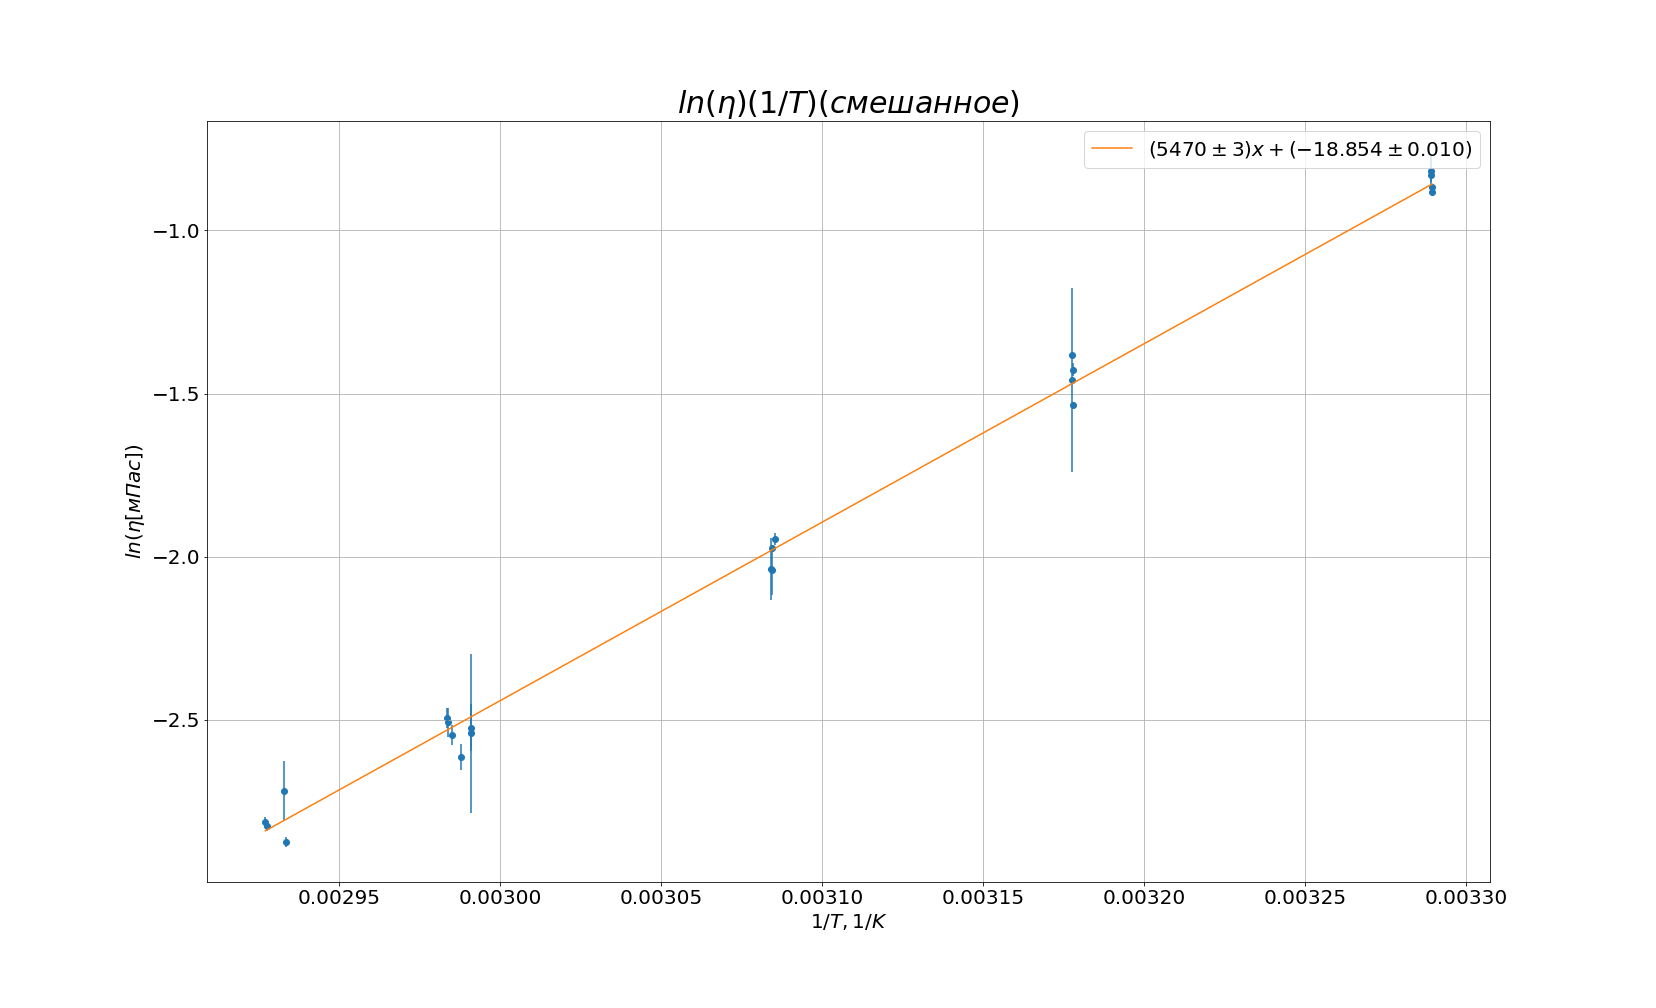
\includegraphics[width=1.2\textwidth]{mixed}
        \label{plot_mixed}
        \caption{График со всеми шариками}
    \end{sidewaysfigure}

    \section{Ссылки }
    [1] Abel G.M.Ferreira, Ana P.V.Egas, Isabel M.A.Fonseca - The viscosity of glycerol, http://dx.doi.org/10.1016/j.jct.2017.05.042
\end{document}



